\documentclass[acmsmall, screen, authorversion, nonacm]{acmart}

\usepackage{listings}
\usepackage{xcolor}

\definecolor{codegreen}{rgb}{0,0.6,0}
\definecolor{codegray}{rgb}{0.5,0.5,0.5}
\definecolor{codepurple}{rgb}{0.58,0,0.82}
\definecolor{backcolour}{rgb}{0.95,0.95,0.92}

\lstdefinestyle{mystyle}{
    backgroundcolor=\color{backcolour},   
    commentstyle=\color{codegreen},
    keywordstyle=\color{magenta},
    numberstyle=\tiny\color{codegray},
    stringstyle=\color{codepurple},
    basicstyle=\ttfamily\footnotesize,
    breakatwhitespace=false,         
    breaklines=true,                 
    captionpos=b,                    
    keepspaces=true,                 
    numbers=left,                    
    numbersep=5pt,                  
    showspaces=false,                
    showstringspaces=false,
    showtabs=false,                  
    tabsize=2
}

\lstset{style=mystyle}

%%
%% \BibTeX command to typeset BibTeX logo in the docs
\AtBeginDocument{%
  \providecommand\BibTeX{{%
    Bib\TeX}}}

\setcopyright{none}

\usepackage{dirtytalk}

%%
%% end of the preamble, start of the body of the document source.
\begin{document}

\title{A Brief History of Rasterized Shadow Algorithms}

\author{Vincent Marias}
\email{vmarias@mines.edu}
\orcid{0009-0003-0991-3180}
\affiliation{%
  \institution{Colorado School of Mines}
  \city{Golden}
  \state{Colorado}
  \country{USA}
}

\begin{abstract}
  I present an overview of three of the most popular shadowing algorithms for real-time rasterized applications, in chronological order as they were introduced/peaked in popularity/viability. I also give implementation details and techniques to improve the results from each algorithm, along with considerations for the benefits and drawbacks of each. The final result is a simple implementation of shadow mapping using percentage-closer filtering, suitable for simple scenes. The introduction additionally contains a brief overview of the broad categories of computer-generated shadows and the rendering equation.
\end{abstract}

\begin{teaserfigure}
  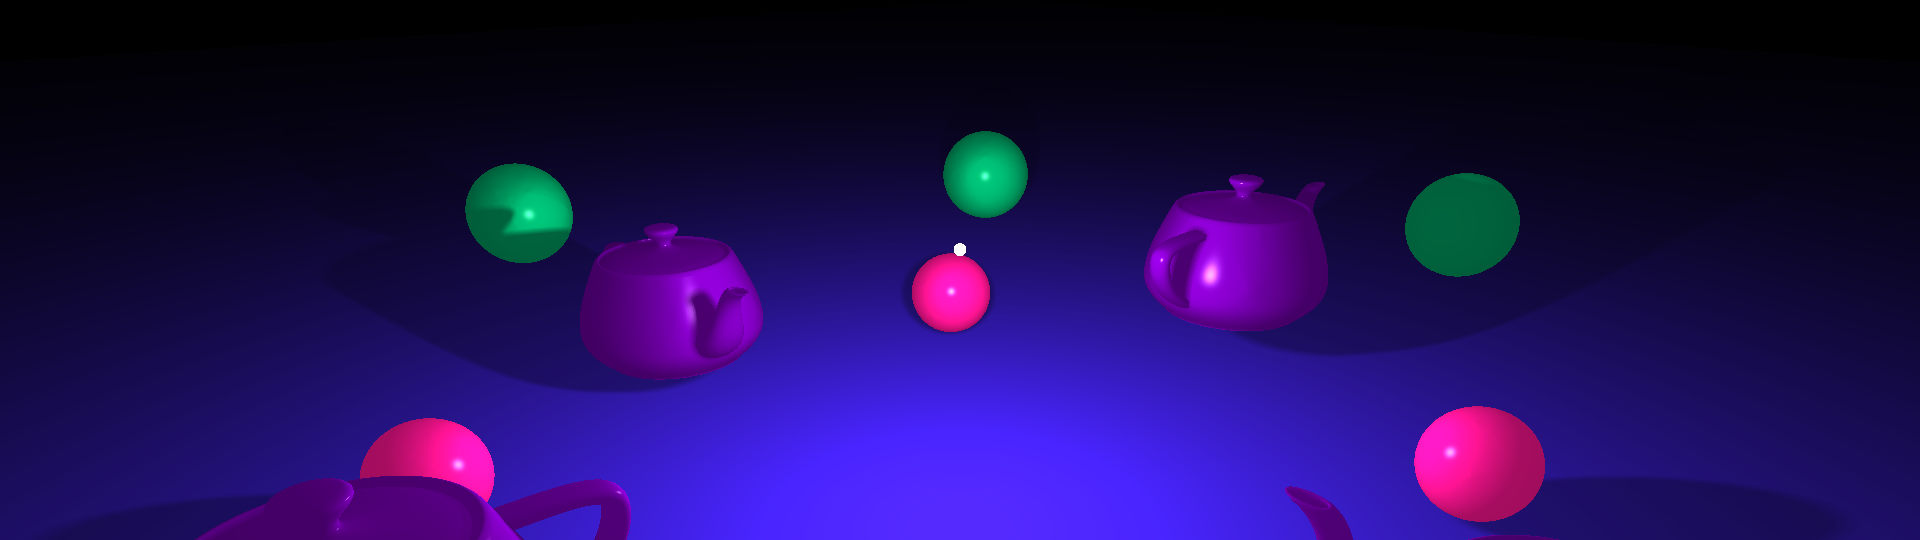
\includegraphics[width=\textwidth]{images/teaser}
  \label{fig:teaser}
\end{teaserfigure}

%%
%% This command processes the author and affiliation and title
%% information and builds the first part of the formatted document.
\maketitle

\section{Introduction}

When rendering a scene, shadows are one of the most important effects that can be added if the goal for the image is realism. They are an integral part of approximating real-world lighting, as much as radiance itself. However, they have long been a sticking point for computer graphics programmers, as the way light is "faked" under rasterization does not facilitate the creation of shadows. To understand why, we'll briefly define shadows and their various computer-generated forms.

\begin{figure}[h]
  \centering
  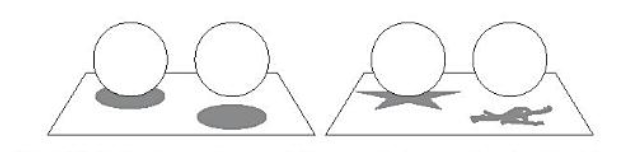
\includegraphics[width=\linewidth]{images/spatial}
  \caption{Shadows have an important influence on the interpretation of spatial relationships in a scene (left). Nevertheless, even course approximations can achieve the same effect (right). \cite{eisemann2011real}}
\end{figure}

What is a shadow? The authors of "Real-Time Shadows" propose a general definition:\newline

\say{An area that is not or is only partially irradiated or illuminated because of the interception of radiation by an opaque object between the area and the source of radiation.} \cite{eisemann2011real}\newline

The most important part of this definition, and the aspect that makes rendering realistic shadows so difficult is the possibility that shadowed areas may be "only \textbf{partially} irradiated". This leads to the two categories of shadows that we can render.

\subsection{Soft Shadows}

In order to fulfill the definition above, we need to render what are called \textbf{soft shadows} in our scene. The basic idea is quite intuitive, given our inate understanding of how light works in the real world. Some shadows are sharp and well-defined, almost a colorless reflection of the object casting them, and some are soft, with blurred edges with difficult-to-define borders. The general difference can be seen in figure 2.

\begin{figure}[h]
  \centering
  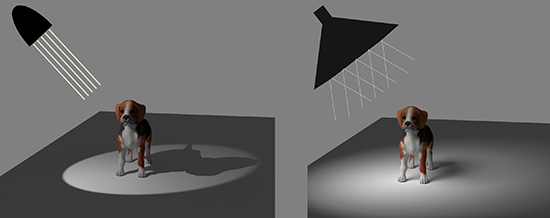
\includegraphics[width=\linewidth]{images/dog}
  \caption{Hard shadows produced by a spotlight (left) vs. soft shadows produced by an area light (right).}
\end{figure}

The darkest part in the middle of a soft shadow is called the \textbf{umbra}, while the softer part around the edges of the umbra is called the \textbf{penumbra}. We'll see why these different parts occur shortly. (There is also the \textbf{antumbra}, but we'll ignore that for our purposes here.)

You'll notice another important difference in the image: the type of light in the scene. Hard shadows are produced by point lights, while soft shadows are produced by area lights.

Consider the scene as a collection of points, either part of an object, \textbf{view samples}, or part of a light source, \textbf{light samples}. We'll call the objects that block light to cast shadows \textbf{casters}, \textbf{occluders}, or \textbf{blockers}, and the objects that have shadows cast onto their surfaces \textbf{receivers}. With this setup, and considering the rendering equation\cite{akenine2019real}, we can start to see how soft shadows can be realised.

\begin{equation}
  L_o \left(\textbf{p}, \omega\right) = L_e(\textbf{p}, \omega) + \int_{\Omega_+}{f_r\left(\textbf{p}, \omega, \hat{\omega}\right) L_i\left(\textbf{p}, \hat{\omega}\right) \cos\left(\textbf{n}_p, \hat{\omega}\right) }\,d\hat{\omega}
\end{equation}

Without going into detail, all we really need to understand about this equation is that for each view sample \begin{math} \textbf{p} \end{math}, we integrate all incoming light \begin{math} L_i \end{math} from every incoming direction \begin{math} \hat{\omega} \end{math} in the hemisphere above that point \begin{math} \Omega_+ \end{math}. One way to think about this is that view samples are lit based on whether or not they "see" one or more light samples. If it sees all the light samples, that point is lit completely by direct light. If it sees none, it is lit only indirectly, and is part of the shadow's umbra. If it sees only some of the light samples, it is paritally lit, and is part of the shadow's penumbra. This integral can be approximated in a rendering application as a summation of some number of sampled view directions.

\subsection{Hard Shadows}

It quickly becomes apparent that approximating soft shadows is extremely difficult due to the expensive calculations that must be performed. Since every light in the real world is an area light - point lights don't really exist - every shadow in the real world is a soft shadow. So in order to render shadows that in any way approach realism, we need soft shadows. But if you remember back to figure 1, we don't actually need realistic shadows to get most of the benefits that shadows in general bring. Even bad shadows are better than no shadows.

This brings us to \textbf{hard shadows}, which are produced by point lights and consist only of the shadow's umbra. These are much easier to compute, and allow us to take advantage of rasterization tricks to generate them in real time.

\section{Related Work}

Many, many researchers have written about shadows and proposed many, many algorithms to render them. In fact, the sheer number of different algorithms and techniques is overwhelming to the point where entire books have been written, such as "Real-Time Shadows"\cite{eisemann2011real}, whose sole purpose is to gather and consolidate as many of the useful ones as possible. The most popular ones are described below in chronological order.

\subsection{Planar Projection Shadows}

In the beginning, there were projection matrices. The perspective projection is one of the fundamental building blocks of rasterization. It projects 3D points from camera space to view space - actual pixel locations on the screen - in a way similar to how the human eye or a pinhole camera works. Another way to think of this is that we project a 3D object onto a 2D image plane. In 1988, Jim Blinn realized that if we consider the scenario of projecting a shadow onto a flat plane, this is very similar to the projection of objects onto the flat image plane\cite{blinn88}. He proposed a technique using a special projection matrix \begin{math} M \end{math}, given a plane defined by the equation \begin{math} \textbf{n} \cdot \textbf{x} + d = 0 \end{math} and a point light at position \begin{math} l \end{math}:

\begin{equation}
  M = 
  \begin{bmatrix}
  \textbf{n} \cdot \textbf{l} + d - \textbf{n}_x \textbf{l}_x & -\textbf{n}_y \textbf{l}_x & -\textbf{n}_z \textbf{l}_x & -d \textbf{l}_x \\
  -\textbf{n}_x \textbf{l}_y & \textbf{n} \cdot \textbf{l} + d - \textbf{n}_y \textbf{l}_y  & -\textbf{n}_z \textbf{l}_y & -d \textbf{l}_y \\
  -\textbf{n}_x \textbf{l}_z & -\textbf{n}_y \textbf{l}_z & \textbf{n} \cdot \textbf{l} + d - \textbf{n}_z \textbf{l}_z & -d \textbf{l}_z \\
  -\textbf{n}_x & -\textbf{n}_y & -\textbf{n}_z & \textbf{n} \cdot \textbf{l}
  \end{bmatrix}
\end{equation}

This generally allows us to project a flat image of any blocker object onto a flat plane on a receiver object. If we then draw this image in black, we have a perfectly sharp hard shadow!

There are some caveats, of course. Blockers and receivers must be separated - no self-shadowing is possible. Receivers must be perfect planes (or parts of a plane). Blockers must be between the light source and the plane, or strange artifacts called anti-shadows will be produced. All blocker geometry is drawn twice, as the shadows are literally flat geometry. But it's simple and fast, which made this an extremely popular technique in real-time applications like games for many years\cite{akenine2019real}.

\subsection{Shadow Textures}

An extension of projection shadows\cite{akenine2019real}, shadow textures start by generating the projections in two passes. Let's think about the process differently, though. If we imagine a camera located at the light source and facing in the direction that light is emitted, we could render the scene from this perspective. In this first pass, render the blockers into a texture. Now, in the second pass, render the receivers while sampling from the texture to determine which fragments are lit and which are in shadow.

This simple method allows for more flexibility: Now we can project shadows onto curved surfaces. However, blockers and receivers are still separated, and now we have to deal with all the problems that come along with textures. Shadow quality becomes an exercise in choosing the best resolution and filtering method for your textures. We'll see what this looks like later, but it's safe to say it was massively over\textbf{shadowed} by the following technique.

\subsection{Shadow Mapping}

By far the most popular and long-lived technique for real-time shadows\cite{akenine2019real}, shadow mapping is a further extension of the shadow textures method. With that method, the texture produced is binary - any fragment is either shadowed or not. The reason this prevents self-shadowing is because if we were to render the blockers again in the second pass, we'd end up deciding that the whole object is in shadow (shadowed by itself). Textures can hold lots more information, so what information are we missing? This technique proposes that we include the depth of each fragment in our texture\cite{williams78}.

Now the process becomes slightly different. In the first pass, we render our texture, but instead of just the blockers, we render every fragment in the scene, recording it's depth. In the second pass, we sample from this texture again. However, we must now calculate the fragment's distance to the light source, and compare this to the stored depth in the texture. If the fragment is closer than that in the texture, it is lit. Otherwise, it is in shadow. This involved transforming each fragment to light space again in the second pass.

Now we have a general, per-fragment solution to hard shadows. Self-shadowing is a given, and point lights can be modeled with ease. However, there are many artifacts that will be discussed later, which arise from the fact that we are now effectively performing a signal reconstruction from a relatively low-resolution signal. Many shadow techniques are simply approaches to mitigating these artifacts\cite{eisemann2011real}.

\section{Problem Statement}

My code implements all three of the above techniques, along with various solutions to each of their shortcomings. I encountered and (at least somewhat) solved all of the artifacting and issues described above. We'll see this in more detail in a moment.

One of the biggest challenges when it comes to both shadow textures and shadow mapping is that of omnidirectional point lights. Of course, a point light is just that: a point. It emits light uniformly in all directions. However, you'll notice that the above techniques only seem to account for what is effecitvely a spot light - the light shining in a single direction (that being the direction our "camera" faces in the first pass). There are a couple of solutions to this, which will also be discussed below.

\section{Problem Solution}

I wrote an OpenGL program capable of rendering spheres, quads, and Utah Teapots. I then constructed a scene with a number of teapots and spheres hovering in a circle above a ground quad, along with a single white point light in the middle of the circle, so that it might cast shadow outwards. The program allows for testing of all three of the following algorithms, as well as real-time adjustment of their parameters.

\subsection{Planar Projection Shadows}

This technique was relatively easy to implement, especially in it's naive form. I send the normal of the plane I want to project onto from the CPU to the GPU via a uniform. In the vertex shader, I apply the above projection matrix (2) to the vertex positions of the blocker objects between the model and projection matrices. Then in the fragment shader, I draw those fragments in black with no transparency. The initial result can be seen in the first image of figure 3. There are some z-fighting issues thanks to drawing directly on top of the ground plane, which are fixed in the second image by turning off the depth test when rendering the shadows. These are still completely black, but if we simply turn on blending, there are layering issues that can be seen in image 3. This is because the shadow itself is literally duplicated geometry, and multiple vertices get projected to the same points. This is more difficult to fix. My solution was to first render the ground plane into the stencil buffer, setting the covered values to 1. Then when drawing the shadows, we can increment any overlaps in the stencil buffer and set up the stencil test so that further overlaps will fail the test - this means shadow fragments are only ever drawn once. Before this addition, the technique could be done in one pass, but with it place, I had to use two passes.

Notice that all the curved objects cast shadow, but only the ground plane can ever receive shadow.

\begin{lstlisting}[language=C]
  // when drawing the receivers (ground plane)
  glEnable(GL_STENCIL_TEST);
  glStencilFunc(GL_ALWAYS, 0, 0xffff);
  glStencilOp(GL_KEEP, GL_INCR, GL_INCR);

  // when drawing the shadows
  glDisable(GL_DEPTH_TEST);
  glStencilFunc(GL_EQUAL, 1, 0xffff);
  glStencilOp(GL_KEEP, GL_INCR, GL_INCR);
\end{lstlisting}

\begin{figure}
	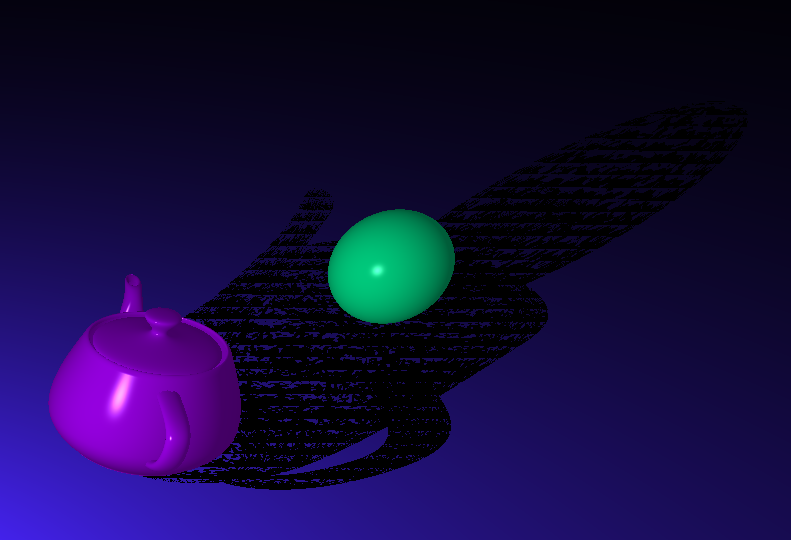
\includegraphics[width=.49\linewidth]{images/planar_1}\hfill
	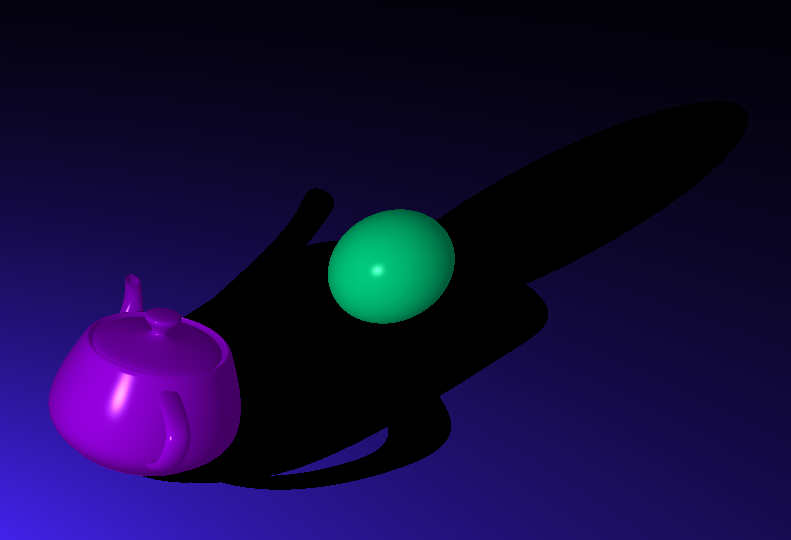
\includegraphics[width=.49\linewidth]{images/planar_2}
	\\[\smallskipamount]
	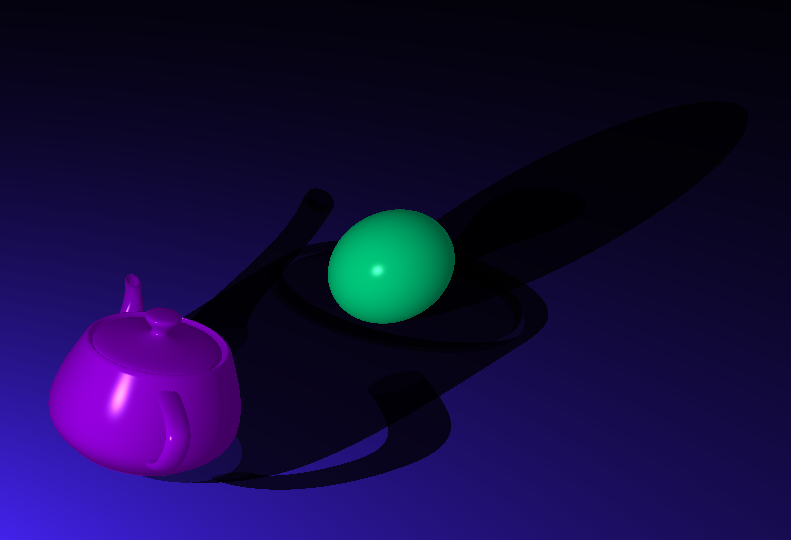
\includegraphics[width=.49\linewidth]{images/planar_3}\hfill
	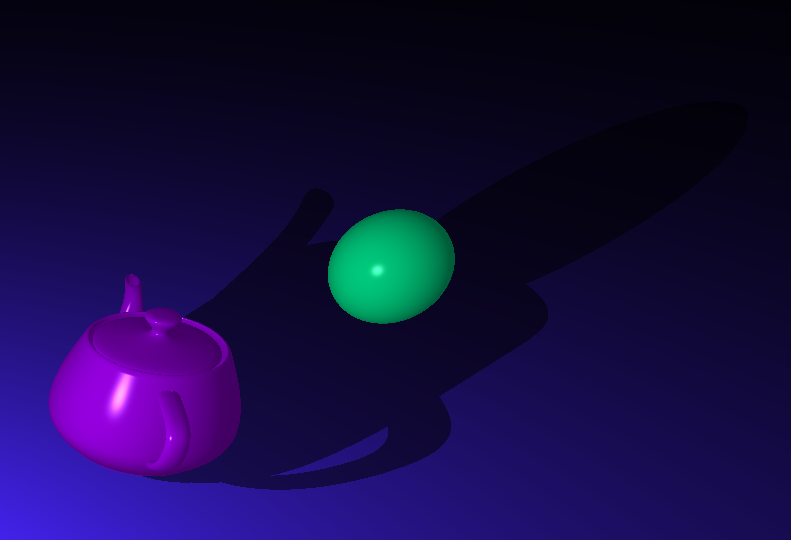
\includegraphics[width=.49\linewidth]{images/planar_4}
	\caption{Naive planar projection shadows displaying z-fighting (top left), with no blending (top right), with naive blending displaying layering (bottom left), and with proper blending via the stencil buffer (bottom right).}
\end{figure}

\subsection{Shadow Textures}

For this technique, I needed to render the scene from the light's perspective. There was the aformentioned issue with rendering in all directions, though. From my research, there are generally two ways to do this. What we need is not a single 2D texture, but a cubemap. So you could render the scene in 6 extra passes, one facing in each direction from the light's perspective and with a square aspect ratio. Or, you construct the cubemap on the fly in the geometry shader to do everything in one pass. It sounds like the second option would be much more efficient, but it turns out that this actually makes the geometry shader very heavy \cite{de2015learn, akenine2019real}, so the performance tradeoff is not so clear. I chose the more simple option of creating the cubemap on the CPU and rendering in seven passes total.

As you can see in the first image, with a low resolution texture (even one-to-one with the final image), the result is not very appealing. Increasing the texture resolution improves things quite a bit, but has a heavy performance cost.

You'll notice that now we can cast shadows onto curved surfaces as well as planes, though to do this we still have to choose which objects are blockers and which are receivers (the green spheres are now receivers and do not cast shadows).

\begin{figure}
	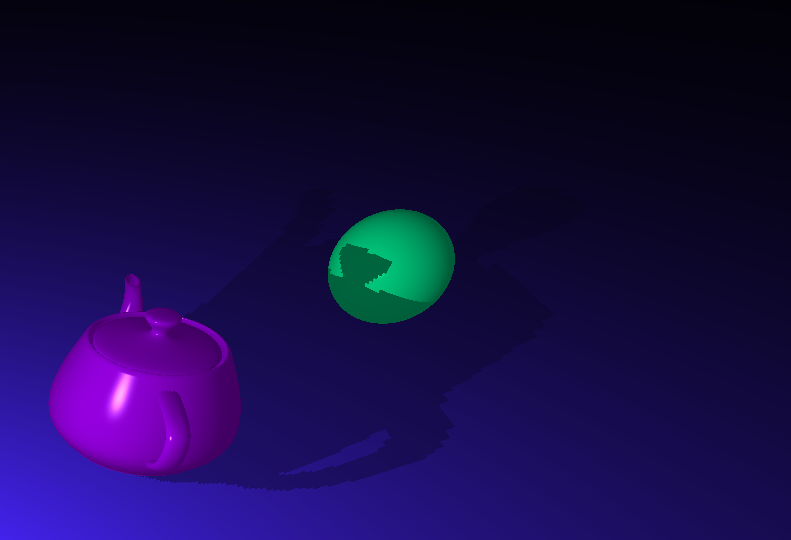
\includegraphics[width=.49\linewidth]{images/textures_1}\hfill
	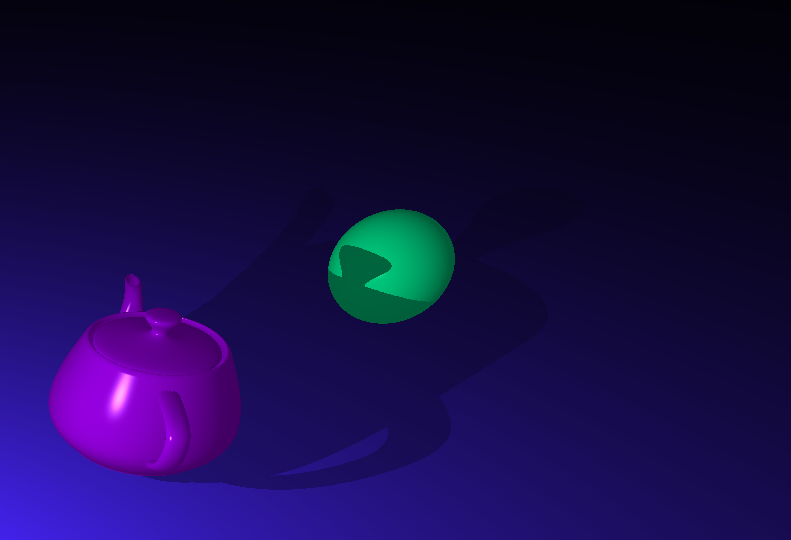
\includegraphics[width=.49\linewidth]{images/textures_2}
	\caption{Low-resolution shadow textures (left) vs. high-resolution (right).}
\end{figure}

\subsection{Shadow Mapping}

With the cubemap and texture write/read framework in place from the previous method, implementing shadow maps was trivial. I simply modified the fragment shader that produces the cubemap (and the texture setup on the CPU) to write the depth component instead of just black. Then in the fragment shader that draws the second pass, I calculate the linear distance\cite{de2015learn} from the fragment to the light source, and use the vector from the light source to the fragment to sample from the cubemap. I then compare the depth value stored there to the calculated distance to determine if the fragment is in shadow or not.

The result can be seen in the first image of figure 5. The artifacts seen there are called \textbf{shadow acne}, and are caused, in a similar manner to z-fighting, by sampling from a discrete texture with a discrete resolution. To fix this, I simply add a small bias to the depth I sample from the cubemap, so the shadows are slightly offset from where they should be but it resolves the acne quite nicely (image 2).

Notice now that all objects are casters and recievers, and objects like the teapot are able to self-shadow. The texture resolution still causes aliasing issues around the edges of the shadows, but we'll resolve that in a moment.

\begin{figure}
	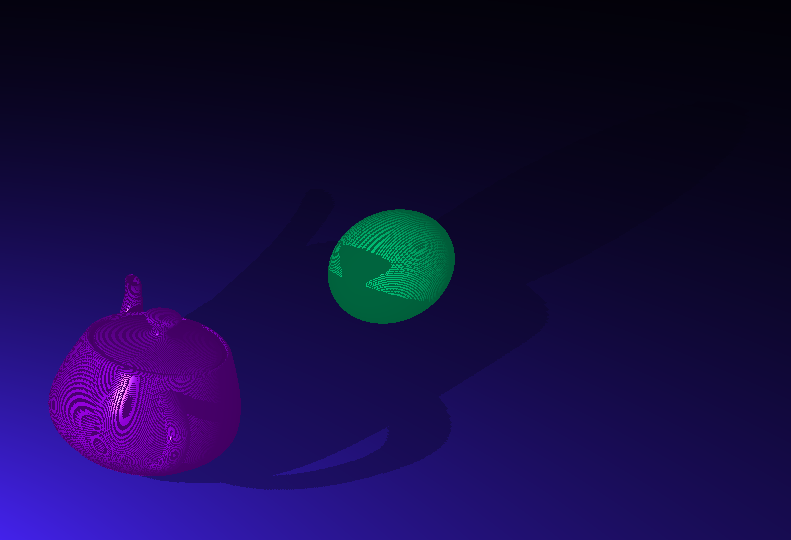
\includegraphics[width=.49\linewidth]{images/maps_1}\hfill
	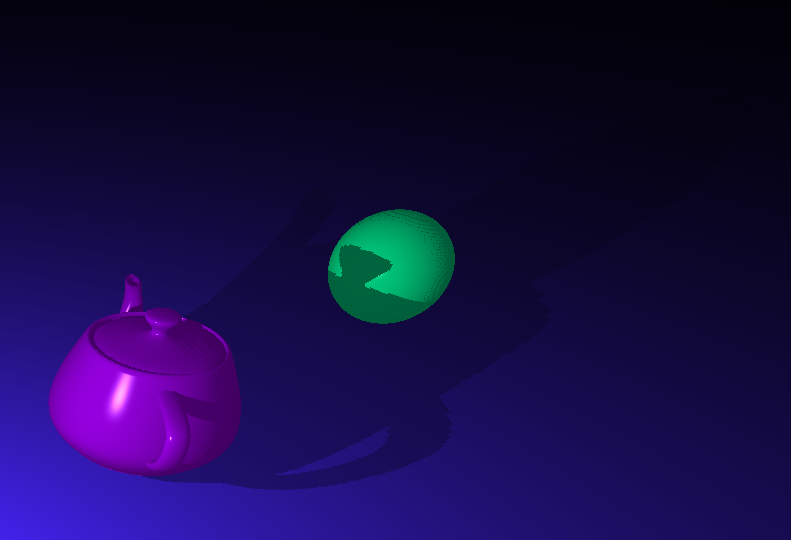
\includegraphics[width=.49\linewidth]{images/maps_2}
	\caption{Naive shadow maps exhibiting acne (left) vs. using a slight depth bias to resolve the acne (right).}
\end{figure}

\subsection{Percentage-Closer Filtering}

The easiest way to resolve the aliasing issues exhibited above is to increase the texture resolution, but this gets expensive very quickly. Instead, let's use some clever filtering to smooth out the result. We can apply a basic filtering kernel to the texture which in it's most simple form just averages the depths of surrounding fragments. By adjusting both the number of samples and the texture resolution, we can obtain quite a nice looking image with very little performance overhead.

There are more advanced kernels you could apply, such as Poisson-Disk Sampling, but for this simple scene their added complexity would not be worth the negligble benefits.

\begin{figure}
	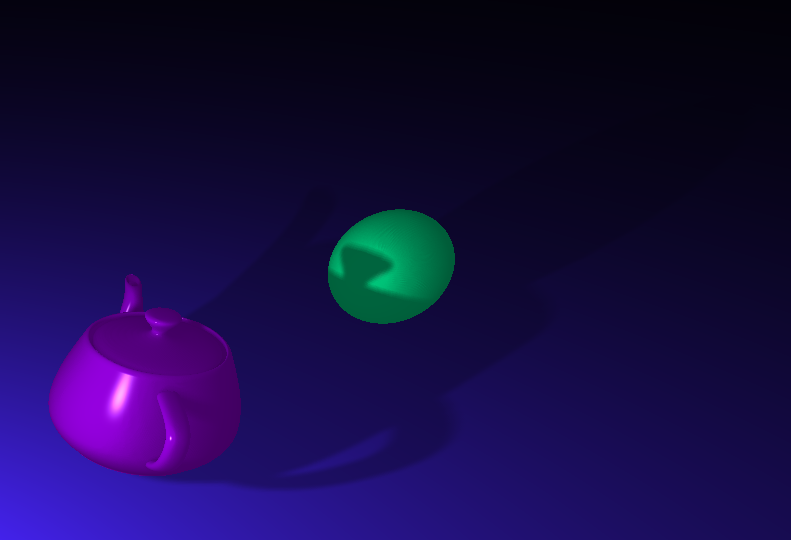
\includegraphics[width=.49\linewidth]{images/pcf_1}
	\caption{Using percentage-closer filtering to reduce aliasing and soften shadow maps.}
\end{figure}

\section{Results}

All of the results can be seen above, but figure 7 contains a wider shot of the scene with the highest-quality shadows I was able to produce by adjusting all the different parameters.

\begin{figure}
	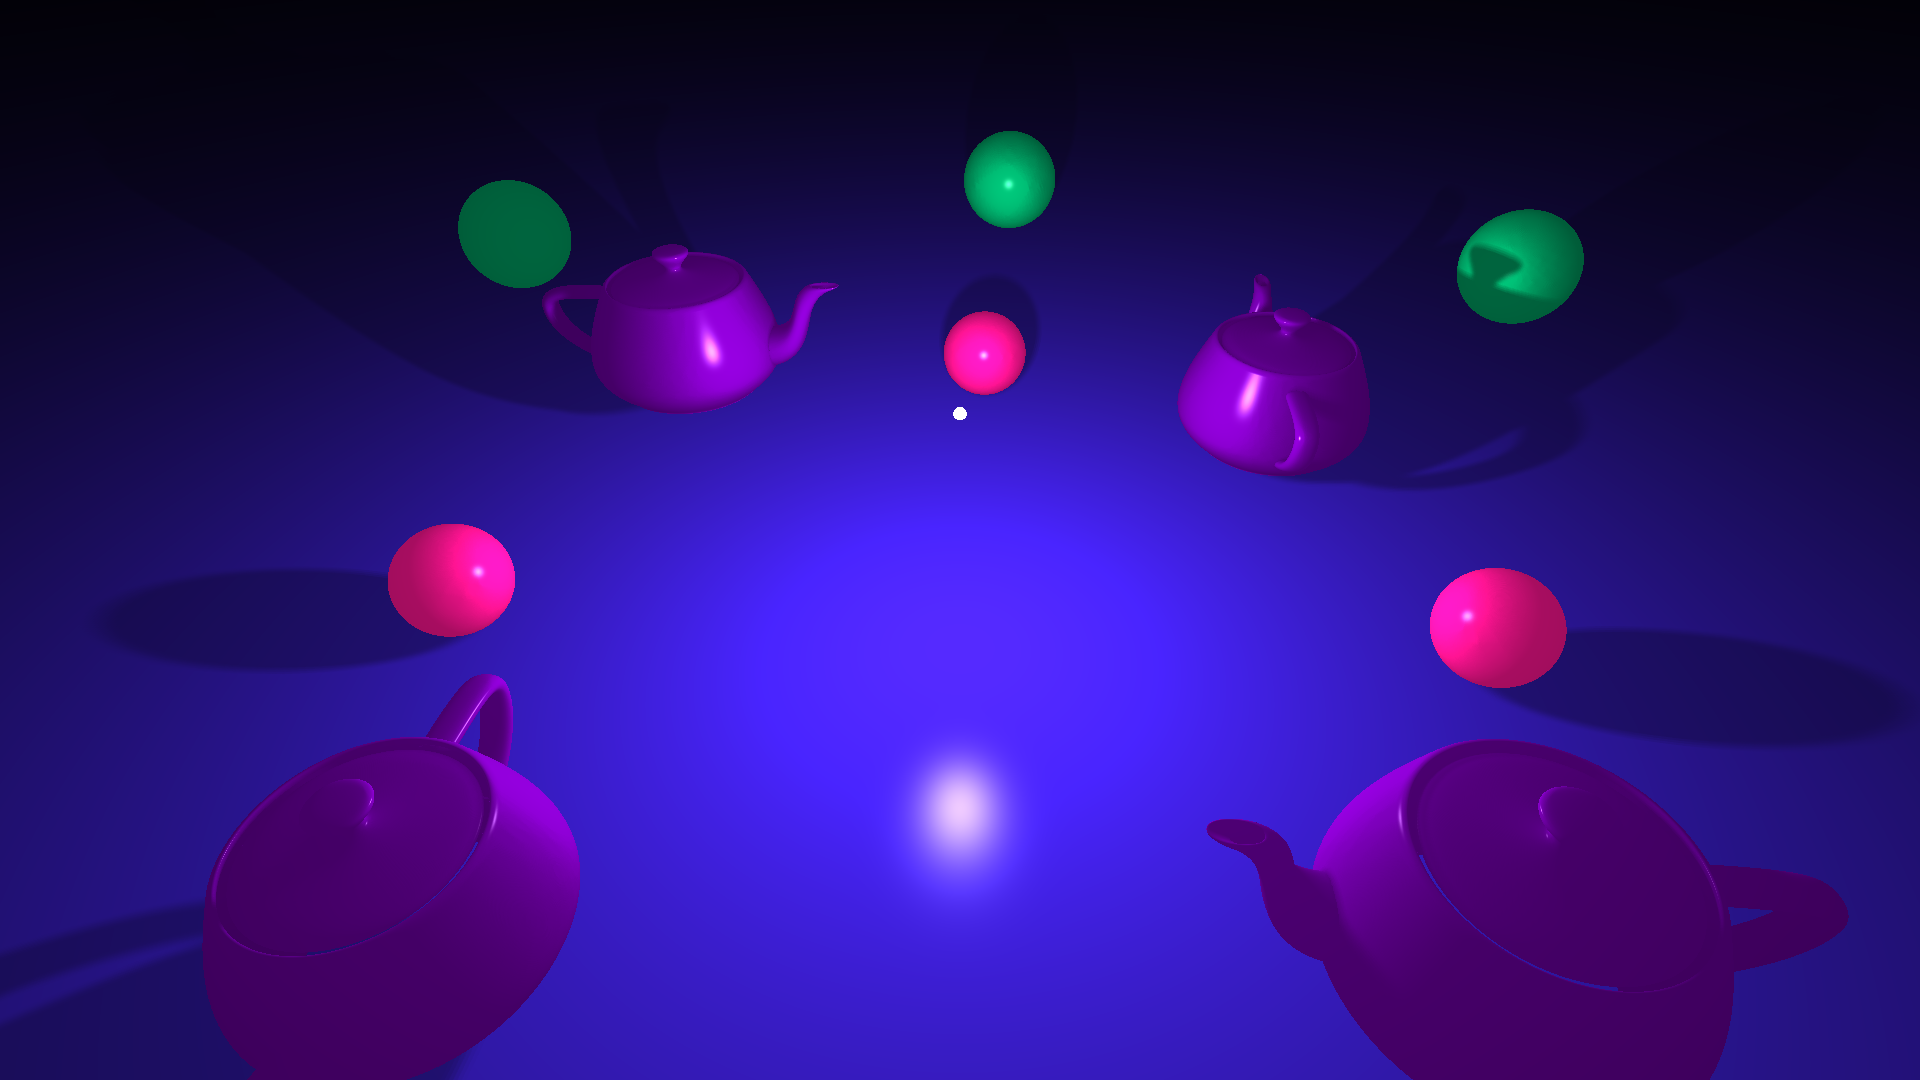
\includegraphics[width=\linewidth]{images/pcf_2}
	\caption{Nice view of the whole scene using shadow maps and PCF.}
\end{figure}

\section{Conclusion}

Through the above results, we can see a progression of shadowing algorithms from very basic and limited to (almost) completely general. Each method brings it's own set of challenges and drawbacks, but none that can't be at least somewhat overcome with rasterization trickery. The most general algorithm - shadow mapping - comes with with largest set of artifacts and issues. Many of these can be alleviated with simple approaches, but to shadow very complex scenes in a convincing and visually appealing way requires much more work. There is endless research on this topic, and an endless number of approaches\cite{eisemann2011real}. Luckily, for simple scenes like the one I constructed for this demonstration, a simple filtering kernel and some careful adjustments are all that's needed for a relatively clean image.

There are still many more techniques not explored here, such as shadow volumes, which also take into account per-object information rather than simply per-fragment. There are also methods to simulate more advanced shadow scenarios, such as shadows cast by semi-transparent objects, shadows cast through media such as fog, or by multi-colored lights. These are outside the scope of this project, however.

I had much grander plans for this project, but writing a polished program to show off the above techniques proved to be more work than I expected. Regardless, I think the final results look quite good.


\bibliographystyle{ACM-Reference-Format}
\bibliography{sources}

\end{document}
\endinput

%%
%% End of file `final-report.tex'.
